%%% Hlavní soubor. Zde se definují základní parametry a odkazuje se na ostatní části. %%%

%% Verze pro jednostranný tisk:
% Okraje: levý 40mm, pravý 25mm, horní a dolní 25mm
% (ale pozor, LaTeX si sám přidává 1in)
\documentclass[12pt,a4paper]{report}
\setlength\textwidth{145mm}
\setlength\textheight{247mm}
\setlength\oddsidemargin{15mm}
\setlength\evensidemargin{15mm}
\setlength\topmargin{0mm}
\setlength\headsep{0mm}
\setlength\headheight{0mm}
% \openright zařídí, aby následující text začínal na pravé straně knihy
\let\openright=\clearpage

%% Pokud tiskneme oboustranně:
% \documentclass[12pt,a4paper,twoside,openright]{report}
% \setlength\textwidth{145mm}
% \setlength\textheight{247mm}
% \setlength\oddsidemargin{15mm}
% \setlength\evensidemargin{0mm}
% \setlength\topmargin{0mm}
% \setlength\headsep{0mm}
% \setlength\headheight{0mm}
% \let\openright=\cleardoublepage

%% Použité kódování znaků: obvykle latin2, cp1250 nebo utf8:
\usepackage[utf8]{inputenc}

%% Ostatní balíčky
\usepackage{graphicx}
\usepackage{amsthm}

%% Balíček hyperref, kterým jdou vyrábět klikací odkazy v PDF,
%% ale hlavně ho používáme k uložení metadat do PDF (včetně obsahu).
%% POZOR, nezapomeňte vyplnit jméno práce a autora.
\usepackage[unicode]{hyperref}   % Musí být za všemi ostatními balíčky
\hypersetup{pdftitle=Název práce}
\hypersetup{pdfauthor=Martin Adam}

%%% Drobné úpravy stylu

% Tato makra přesvědčují mírně ošklivým trikem LaTeX, aby hlavičky kapitol
% sázel příčetněji a nevynechával nad nimi spoustu místa. Směle ignorujte.
\makeatletter
\def\@makechapterhead#1{
  {\parindent \z@ \raggedright \normalfont
   \Huge\bfseries \thechapter. #1
   \par\nobreak
   \vskip 20\p@
}}
\def\@makeschapterhead#1{
  {\parindent \z@ \raggedright \normalfont
   \Huge\bfseries #1
   \par\nobreak
   \vskip 20\p@
}}
\makeatother

% Toto makro definuje kapitolu, která není očíslovaná, ale je uvedena v obsahu.
\def\chapwithtoc#1{
\chapter*{#1}
\addcontentsline{toc}{chapter}{#1}
}

\begin{document}

% Trochu volnější nastavení dělení slov, než je default.
\lefthyphenmin=2
\righthyphenmin=2

%%% Titulní strana práce

\pagestyle{empty}
\begin{center}

\large

Charles University in Prague

\medskip

Faculty of Mathematics and Physics<

\vfill

{\bf\Large BACHELOR THESIS}

\vfill

\centerline{\mbox{
\includegraphics[width=60mm]{img/logo.eps}}}

\vfill
\vspace{5mm}

{\LARGE Martin Adam}

\vspace{15mm}

% Název práce přesně podle zadání
{\LARGE\bfseries Title of the thesis}

\vfill

% Název katedry nebo ústavu, kde byla práce oficiálně zadána
% (dle Organizační struktury MFF UK)
Name of the department or institute

\vfill

\begin{tabular}{rl}

Supervisor of the bachelor thesis: & First and last name \\
\noalign{\vspace{2mm}}
Study programme: & programme \\
\noalign{\vspace{2mm}}
Specialization: & specialization \\
\end{tabular}

\vfill

% Zde doplňte rok
Prague 2015

\end{center}

\newpage

%%% Následuje vevázaný list -- kopie podepsaného "Zadání bakalářské práce".
%%% Toto zadání NENÍ součástí elektronické verze práce, nescanovat.

%%% Na tomto místě mohou být napsána případná poděkování (vedoucímu práce,
%%% konzultantovi, tomu, kdo zapůjčil software, literaturu apod.)

\openright

\noindent
%TODO
Dedication...

\newpage

%%% Strana s čestným prohlášením k bakalářské práci

\vglue 0pt plus 1fill

\noindent
I declare that I carried out this bachelor thesis independently, and only with the cited
sources, literature and other professional sources.

\medskip\noindent
I understand that my work relates to the rights and obligations under the Act No.
121/2000 Coll., the Copyright Act, as amended, in particular the fact that the Charles
University in Prague has the right to conclude a license agreement on the use of this
work as a school work pursuant to Section 60 paragraph 1 of the Copyright Act.

\vspace{10mm}

\hbox{\hbox to 0.5\hsize{%
In ........ date ............
\hss}\hbox to 0.5\hsize{%
signature of the author
\hss}}

\vspace{20mm}
\newpage

%%% Povinná informační strana bakalářské práce

\vbox to 0.5\vsize{
\setlength\parindent{0mm}
\setlength\parskip{5mm}

Název práce:
Název práce
% přesně dle zadání

Autor:
Martin Adam

Katedra:  % Případně Ústav:
Název katedry či ústavu, kde byla práce oficiálně zadána
% dle Organizační struktury MFF UK

Vedoucí bakalářské práce:
Jméno a příjmení s tituly, pracoviště
% dle Organizační struktury MFF UK, případně plný název pracoviště mimo MFF UK

Abstrakt:
% abstrakt v rozsahu 80-200 slov; nejedná se však o opis zadání bakalářské práce

Klíčová slova:
% 3 až 5 klíčových slov

\vss}\nobreak\vbox to 0.49\vsize{
\setlength\parindent{0mm}
\setlength\parskip{5mm}

Title:
% přesný překlad názvu práce v angličtině

Author:
Martin Adam

Department:
Název katedry či ústavu, kde byla práce oficiálně zadána
% dle Organizační struktury MFF UK v angličtině

Supervisor:
Jméno a příjmení s tituly, pracoviště
% dle Organizační struktury MFF UK, případně plný název pracoviště
% mimo MFF UK v angličtině

Abstract:
% abstrakt v rozsahu 80-200 slov v angličtině; nejedná se však o překlad
% zadání bakalářské práce

Keywords:
% 3 až 5 klíčových slov v angličtině

\vss}

\newpage

%%% Strana s automaticky generovaným obsahem bakalářské práce. U matematických
%%% prací je přípustné, aby seznam tabulek a zkratek, existují-li, byl umístěn
%%% na začátku práce, místo na jejím konci.

\openright
\pagestyle{plain}
\setcounter{page}{1}
\tableofcontents

%%% Jednotlivé kapitoly práce jsou pro přehlednost uloženy v samostatných souborech
\chapter*{Introduction}
\addcontentsline{toc}{chapter}{Introduction}

\section*{The Worldwide LHC Computing Grid}
On the edge of our millennium scientists working on the Large Hadron Collider (LHC) were expecting enormous volumes 
of data, larger then any single computing center within the LHC collaboration could handle, so the concept of 
distributed data management was conceived. In 2001 the CERN\footnote{European Organization for Nuclear Research 
(name derived from Conseil Européen pour la Recherche Nucléaire) -- European research organization that operates 
the largest particle physics laboratory in the world.} Council approved the start of an international 
collaborative project that consists of a grid-based computer network infrastructure, the Worldwide LHC Computing 
Grid (WLCG)~\cite{happyBday}. 

The WLCG has a hierarchical architecture, where participating sites are categorized according to the resources and 
services they provide into four importance levels called Tiers. Each Tier is represented by a single or 
distributed computing and storage cluster and provides a specific set of services. The largest center, CERN data 
center or Tier-0, provides the  permanent storage of experimental data and makes the data available for the WLCG 
processing. Although it provides less than 20\% of the WLCG computing capacity, the role of CERN is unique in 
keeping one copy of the data from all experiments and for performing the first pass of the data reconstruction. 
When LHC is not running, Tier-0 provides resources for re-processing of the raw experimental data and eventually 
for simulation campaigns. 

\begin{wrapfigure}{L}{0.6\textwidth}
\centering
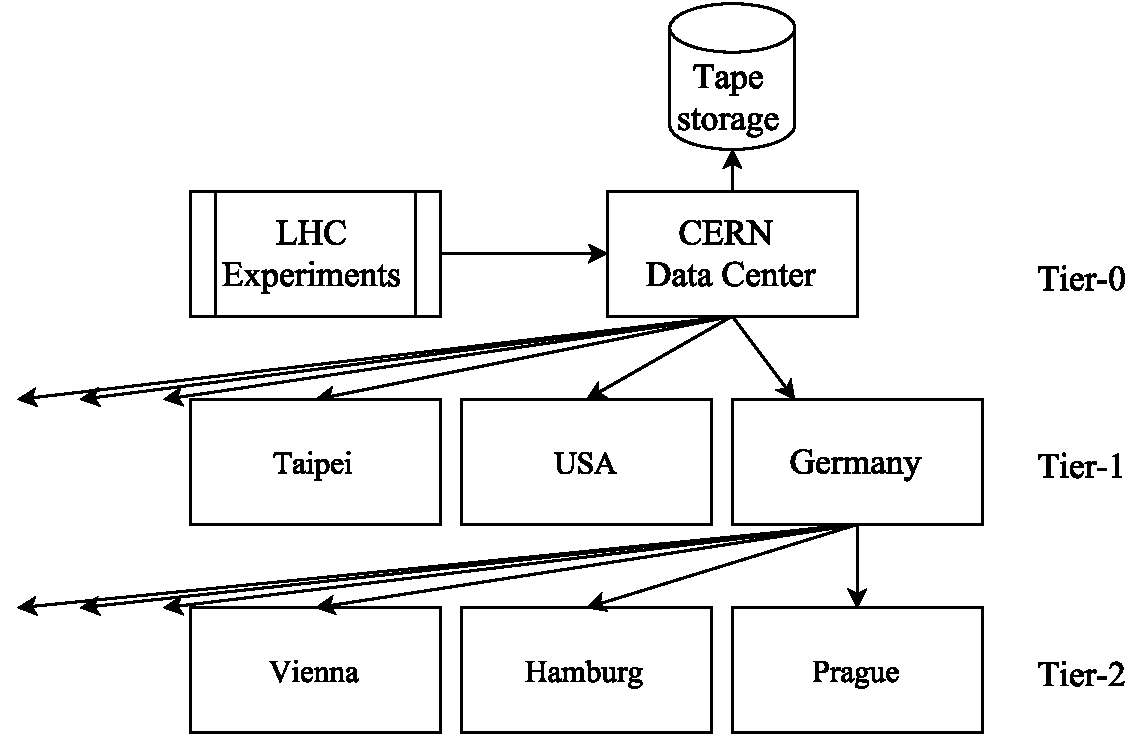
\includegraphics[width=0.55\textwidth]{Tiers.pdf}
\caption{The WLCG Tier-1 centers with CERN Tier-0 in the middle}
\label{fig:WLCG}
\end{wrapfigure}

Another copy is passed to one of the Tier-1 centers. Tier-1s are huge computing centers located in Europe, Canada, USA 
and Taipei. They provide non-stop support for the Grid, store a share of raw data, perform reprocessing and store 
its output. They are connected to CERN with dedicated high-bandwidth optical-fiber links. Then there are more than 
160 Tier-2 centers all around the world. Their role is mainly to run simulation campaigns and end-user analysis. 
Tier-3 centers are small local computing clusters at universities or research institutes and even individual 
PCs~\cite{TGrid}.

\section*{Grid Middleware}

The operation and functionality of WLCG, as well as other Grid systems, is enabled by specific software packages 
and protocols, so-called Grid middleware. This manages the basic domains of the Grid functions: job management, 
data management, security and information services \cite{GriCom}. The term middleware reflects the specific role 
of this software packages and protocols system: it is a layer between the application area for solving users tasks 
and the resource area consisting of basic fabric and connectivity layer. 

The vast variety of requirements and needs of the user communities from the four LHC experiments is impossible to 
meet with only one set of middleware components. Consequently, each experiment user group started developing its 
own set of tools, which meet their needs. For example AliEn is a middleware solution made by the 
ALICE\footnote{One of the experiments hosted at CERN} experiment collaboration and DIRAC was developed by the 
LHCb\footnote{Another experiment hosted at CERN} collaboration. Along with some packages from the WLCG-middleware 
they include some additional specific packages and provide complete framework for data processing according to the 
individual experiments' computing models.

\section*{DIRAC}

The DIRAC\footnote{The Distributed Infrastructure with Remote Agent Control} middleware was developed to satisfy
the needs of not only the LHCb collaboration developing it, but also to enable other smaller experiments to use
it as their middleware solution. This was achieved by concentrating on modular architecture, which helps with
adding new features or modifying the systems behavior according to individual experiments needs. 

DIRAC is constructed from loosely coupled systems where each system manages one part of its functionality. This 
thesis concentrates on the DIRAC File Catalog, which is part of the Data Management system. This particular system 
is responsible data managing tasks across a wide range of distributed storage elements. It also enables users to 
quickly find and use their files. This is the goal of the File Catalog. It is accomplished by maintaining a 
directory structure with a similar interface as UNIX shell and enabling users to define their own metadata
and use them to search for files.

\section*{Goals of the Thesis}

The first task of this thesis is to upgrade the DIRAC File Catalog by 
\begin{itemize}
\item adding a new module for dataset support enabling users to bundle their files, based on a metadata search 
(a~metaquery) into a single object,
\item implementing a class to encapsulate all the methods handling metaquery as well as to extend its 
functionality by adding normalization and optimization procedures.
\end{itemize}

%\noindent 
The second task is to test the hypothesis that storing the user defined metadata in a suitable NoSQL database 
would improve metaquery performance. If the tests prove that hypothesis, the task is to extend the code of DIRAC 
to incorporate the database in the File Catalog making a prototype, that can be then evaluated by the DIRAC 
collaboration.

\section*{Structure of the Thesis}

In chapter \ref{chap:DIRAC} the DIRAC middleware will be introduced with focus on the data management part and the 
file catalog. Afterwards DIRAC will be compared to two other middleware solutions in chapter \ref{chap:relwork}, 
more specifically ATLAS Distributed Data Management system and ALICE Environment framework.

In the next two chapters the contribution of this project to DIRACs code will be presented. Chapter \ref{chap:MQ} 
is about the new MetaQuery class and chapter \ref{chap:Dataset} refers about the Dataset Manager.

In the last part several NoSQL databases are tested in order to pick the one that would be the best for storing
file metadata (chapter \ref{chap:databases}) and in chapter \ref{chap:NoSQL} a module created for integrating that 
database is described. 

Finally chapter \ref{chap:user} provides user documentation to all the commands used to interact with the CLI of 
the DFC used to control any of the parts that were changed by this project. The last chapter
provides conclusion as well as evaluation of the test results.
\chapter{The Distributed Infrastructure with Remote Agent Control}

\section{About DIRAC}
The LHCb Collaboration\cite{LHCb} is running one of the four detectors attached to the LHC particle 
collider at CERN, Geneva. The amount of data produced by the experiment
annually is so large that it necessitates the development of a specialized system for the data
production, reconstruction and analysis. The DIRAC project of the LHCb Collaboration was started to
provide such a system.\cite{Dir2} The developers were aiming to create a easy to run system, seamlessly using 
the various heterogeneous computing resources available to the LHCb Collaboration, that can be run by only one 
production manager. 

The DIRAC software architecture is based on a set of distributed, collaborating services. Designed to have a
light implementation, DIRAC is easy to deploy, configure and maintain on a variety of platforms. Following
the paradigm of a Services Oriented Architecture (SOA), DIRAC is lightweight, robust and scalable. Because one 
of the primary goals was to support various virtual organization with their specific needs, it supports well 
isolated plugable modules, where the organizations specific features can be located. It allows to construct medium
sized grids of up to several thousands processors by integrating diverse resources within its integrated Workload
Management System. The DIRAC Data Management components provide access to standard grid storage systems based 
on the SRM standard interface \cite{SRM} or ordinary (S)FTP, HTTP file servers. The File Catalog options include the
LCG File Catalog (LFC) as well as a simple DIRAC File Catalog, discussed later. 

\subsection{DIRAC architecture}
DIRAC components can be grouped in to 4 categories: 
\begin{description}

\item[Resources] \hfill \\
Resources are components which provide access to the computing and storage facilities available to
DIRAC. Computing resources include individual PCs, computer farms, cloud resources and computing grids. Storage 
resources include storage elements with SRM interface and most of the popular data access protocols (gridftp,
(s)ftp, http,...) are integrated as well. DIRAC does not provide a complex storage element, it includes however a 
Storage Element service which provides access to disk storage managed by a POSIX compliant file system.

\item[Services] \hfill \\
The DIRAC system is built around a set of loosely coupled services which keep the system state and
help to carry out workload and data management tasks. The services are passive components which
are only reacting to the requests of their clients possibly soliciting other services in order to
accomplish the requests. Each service has typically a MySQL database backend to store the state
information. The services accept incoming connections from various clients. These can be user interfaces,
agents or running jobs. 

\item[Agents] \hfill \\
Agents are light and easy to deploy software components built around a unified framework. They are active
components, usually deployed close to the corresponding services, watching for changes in the service states and 
reacting accordingly by initiating actions like job submission or result retrieval. 

\item[Interfaces] \hfill \\
The DIRAC functionality is exposed to the system developers and to the users in a variety of ways. 
	\begin{itemize}
	\item The DIRAC programming language is python, so the programming interfaces (APIs) are provided in this 		
		language
	\item For users the DIRAC functionality is available through a command line interface. Some DIRAC subsystems 		
		have specialized shells to work with.
	\item DIRAC also provides a web interface suitable for monitoring and managing the system behavior.
	\end{itemize}

\end{description}

\subsection{Framework}
\cite{DISET}

\section{DIRAC Data Management System}


\section{DIRAC File Catalog}
% what is it
% metadata
% replica catalog


\chapter{Related works}

For comparison we can look for other similar systems as DIRAC. The DFC was made by the LHCb experiment collaboration,
its needs are similar to those of other LHC experiments so the ATLAS Distributed Data Management system and the AliEn 
file catalog would make a good comparison.


\section{ATLAS DDM}
The ATLAS experiment at LHC is a general purpose particle detector designed to investigate physics at the energy
frontier. The output data-rate, already reduced by the online trigger is  200-400Hz. Even with this reduction 
ATLAS records a huge amount of data – more than 8PB of raw collision data have been taken since the LHC
started running. After processing at ATLAS Tier-0s, the data is registered in the ATLAS Distributed Data Management
system (DDM) \cite{ATLASDDM1}. Without deeply studying the implementation of it I would like to take a look 
at its main concepts.

Although a basic unit of data in the ATLAS DDM is a file the basic operational unit is a dataset: they may be
transferred to grid sites, whereas single files may not. There is also one more layer of aggragation called the 
container, which is a collection of datasets. Datasets may overlap and in practice they do so in a 
hierarchical manner: production will use small datasets, referring to a few jobs processed at a site. These datasets
are then aggregated into the main dataset, which refers to a particular task in the ATLAS
production system. Then these main datasets may be added to a container, where the output of several 
similar simulation tasks is gathered. Datasets may be opened (new files can be added to them), closed (no new files
may be added, but could have versions which differ in file content) and frozen (no new files may be added and no 
new versions created). 

The responsibilities of the ATLAS DDM cover data registration, transfers between sites, file deletion, dataset 
consistency ensuring (manage file loses on sites), enforcing ATLAS Computing model policies and monitoring. The
current implementation is called Rucio (previous was DQ2).


\subsection{Rucio}
In this implementation files, datasets and containers follow an identical naming scheme which is composed of the
scope and a name, called a data identifier \cite{ATLAS-Rucio}. Scopes are used to separate production and individual
users. Metadata associated with a data identifier is represented using attributes (e.g. for file its availability,
for dataset whether it is opened, closed or frozen,...) which are key-value pairs. The set of available attributes 
is restricted. Some metadata attributes are user settable, e.g. physics attributes (run number). Non user settable 
metadata include system attributes (size, creation time,...). For datasets and containers it is possible that the 
value of metadata is a function of the metadata of its constituents, e.g. the total size is the sum of the
sizes of the constituents.

A Rucio Storage Element (RSE) is a repository for physical files. It is the smallest unit of
storage space addressable within Rucio. It has an unique identifier and a set of properties (supported protocols,
storage type, physical space,...). Physical files stored on RSEs are identified by their Physical File Name (PFN).
The PFN is a fully qualified path identifying a replica of a file. The mapping between the file identifier and
the PFN is a deterministic function of the identifier, RSE and protocol. Replica management in Rucio is based on
replication rules defined on data identifier sets. A replication rule is owned by an account and defines the 
minimum number of replicas to be available on a list of RSEs.

\section{AliEn}

AliEn (ALICE Environment) is a Grid framework developed by the ALICE
Collaboration and used in production for more than 14 years. Since 2005, AliEn
has been used for both data production and user analysis  \cite{AliEn2}. 

The AliEn File Catalogue is one of the key components in the AliEn system. It
provides the mapping between Logical File Names (LFNs) visible to the end user
and one or more Physical File Names (PFNs) which describe the physical location
of the file by identifying the name of a storage element and the path to the
local file  The LFNs are manipulated by users, one LFN can point to more PFNs.
To prevent duplicate entries, each LFN is associated with a Globally Unique
IDentifier (GUID).
The interface of the catalogue is a hierarchical structure of directories and
files, similar to a UNIX file system. The directories and files in the File
Catalogue have Unix like privileges.
It also extends the familiar file system paradigm to include information about
running processes in the system (in analogy to the /proc directory on Linux
systems). Each job inserted into AliEn Task Queue gets a unique id and a
corresponding /proc/id directory where it can register temporary files,
standard input and output as well as all job products \cite{AliEn1}.
The File Catalogue is designed to allow each directory node in the hierarchy to
be supported by different database engines, possibly running on different hosts
and even having different internal table structures optimized for a particular
directory branch. 
From user point of view, the catalogue behaves as a single entity, internally
it is divided between the LFN and GUID catalogues, which are kept in separate
databases. Every LFN database has an index table used to locate the files and
table that contains all the information about the concrete LFN (owner, group,
size...).
In addition, there could be some user-defined tables containing metadata.
AliEn supports file collections.  A file collection is a user defined list of
entries, which can be ether another collections, LFNs or GUIDs. The collection
looks like a normal file in the file catalogue, its size is the sum of sizes of
all its components. If a command is executed on a collection, it will be
executed on each entry of that collection (e.g. if a user issues a command to
replicate a collection, all the files of that collection will be replicated).

\section{Main differences?}

% Ukázka použití některých konstrukcí LateXu (odkomentujte, chcete-li)
% %%% Ukázka použití některých konstrukcí LaTeXu

\subsection{Ukázka \LaTeX{}u}
\label{ssec:ukazka}

This short subsection serves as an~example of basic \LaTeX{} constructs,
which can be useful for writing a~thesis.

Let us start with lists:

\begin{itemize}
\item The logo of Matfyz is displayed in figure~\ref{fig:mff}.
\item This is subsection~\ref{ssec:ukazka}.
\item Citing literature~\cite{lamport94}.
\end{itemize}

Different kinds of dashes:
red-black (short),
pages 16--22 (middle),
$45-44$ (minus),
and this is --- as you could have expected --- a~sentence-level dash,
which is the longest.
(Note that we have follwed \verb|a| by a~tilde instead of a~space
to avoid line breaks at that place.)

\newtheorem{theorem}{Theorem}
\newtheorem*{define}{Definition}	% Definice nečíslujeme, proto "*"

\begin{define}
A~{\sl Tree} is a connected graph with no cycles.
\end{define}

\begin{theorem}
This theorem is false.
\end{theorem}

\begin{proof}
False theorems do not have proofs.
\end{proof}

\begin{figure}
	\centering
	
\includegraphics[width=30mm]{../img/logo.eps}
	\caption{Logo of MFF UK}
	\label{fig:mff}
\end{figure}


\chapter*{Conclusion}
\addcontentsline{toc}{chapter}{Conclusion}
\label{chap:conc}

This project successfully added dataset support to the DIRAC File Catalog making DIRAC even more 
versatile. Dataset support was actively requested by two experiments, that can now start using DIRAC. 
Closely coupled with the dataset functionality went the development of the new MetaQuery
class that extended the metaquery language by adding more logical operators. The new MetaQuery also
supports normalization and optimization of the query input, opening new possibilities for future usage
in the DIRAC Data Management system as well as in the Workflow Management system. 

This project also tackled the problem of storing metadata. Trying to enhance the current solution, a couple of NoSQL 
databases were tested on sample data similar to the DIRAC production metadata. The tests proved that connecting the 
metadata part of DFC to a NoSQL database could improve query performance, especially on more complex
queries. A better performance is observable when applying 4 and more constraints and retrieving less than 10 000 
hits.

To prove the concept of connecting a NoSQL database to DIRAC, a new module was developed to provide 
a interface between DFC and the database. As the back-end database Elasticsearch was used, because it performed
best in the conducted tests. To improve the query performance, the complexity was moved from the python code of
DIRAC to the database engine. This was traded by adding complexity to the management procedures. These do not have 
to be, unlike the query mechanism, optimized for time performance.

In future if the DIRAC collaboration decides to use Elasticsearch as the database back-end for the metadata
catalog, more functionality can be added using Elasticsearch specific features. 
For example when a query is executed, the number of documents satisfying it is returned before all the documents are 
fetched. This could be used for example when checking the properties of a dynamic dataset or when trying to predict
the time for fetching all the results of a particular query could be. Also new comparison 
operators translating to one of Elasticsearch query 
types\footnote{\url{https://www.elastic.co/guide/en/elasticsearch/reference/current/term-level-queries.html}} can be 
added to extend the metaquery language.

%%% Seznam použité literatury
%%% Seznam použité literatury je zpracován podle platných standardů. Povinnou citační
%%% normou pro bakalářskou práci je ISO 690. Jména časopisů lze uvádět zkráceně, ale jen
%%% v kodifikované podobě. Všechny použité zdroje a prameny musí být řádně citovány.

\def\bibname{Bibliography}
\begin{thebibliography}{99}
\addcontentsline{toc}{chapter}{\bibname}

%\bibitem{lamport94}
%  {\sc Lamport,} Leslie.
%  \emph{\LaTeX: A Document Preparation System}.
%  2. vydání.
%  Massachusetts: Addison Wesley, 1994.
%  ISBN 0-201-52983-1.

\bibitem{happyBday}
	Hayes, Jacqui: 
	\emph{Happy 10th Birthday, WLCG!} [online]
	International Science Grid This Week [ref. 2014-09-18]
	\url{www.isgtw.org/feature/happy-10th-birthday-wlcg}

\bibitem{TGrid}
	\emph{The Grid: A system of tiers} [online] 
	CERN [ref. 2014-09-18]
	\url{home.web.cern.ch/about/computing/grid-system-tiers}

\bibitem{GriCom}
	\emph{Grid Computing - Technology and Applications, Widespread Coverage and New Horizons.} 
	edited by Maad, Soha; InTech, 2012.
	ISBN 978-953-51-0604-3

\bibitem{UI}
	\emph{User Interfaces} [online] 
	EGIWiki [ref. 2014-09-29]
	\url{wiki.egi.eu/wiki/User_Interfaces}
	
\bibitem{LHCb}
	A. A. ALVES, L. M. FILHO, A. F. BARBOSA, I. BEDIAGA, G. CERNICCHIARO, G. GUERRER, H. P. LIMA, A. A. MACHADO, et al. 
	The LHCb Detector at the LHC.
	\textit{Journal of Instrumentation}. 
	2008-08-01, vol.~3, issue 08. 
	DOI: 10.1088/1748-0221/3/08/S08005.
	
\bibitem{Dir2}
	A. TSAREGORODTSEV, M. BARGIOTTI, N. BROOK, et al. 
	DIRAC: a community grid solution. \
	textit{Journal of Physics: Conference Series}. 2008-07-01, vol.~119, issue 6.
	DOI: 10.1088/1742-6596/119/6/062048.
	
\bibitem{SOA}
	T. ERL. 
	\textit{Service-oriented architecture: concepts, technology, and design}. 
	Upper Saddle River, NJ: Prentice Hall Professional Technical Reference, 2005, xxviii, 
	760 p. ISBN 01-318-5858-0.

	
\bibitem{SRM}
	A. SHOSHANI,  A. SIM, J. GU. 
	Storage Resource Managers: Middleware Components for Grid Storage. 
	2002.
	
\bibitem{MySQL}
	P. DUBOIS. \textit{MySQL: the definitive guide to using, programming, and administering MySQL 4.1 and 5.0}. 
	3rd ed. Indianapolis, Ind.: Sams Pub., 2005, xxii, 1294 p. ISBN 06-723-2673-6.

\bibitem{DISET}
	A. CASAJUS,  R. GRACIANI and The Lhcb Dirac TEAM. 
	DIRAC distributed secure framework. 
	\textit{Journal of Physics: Conference Series}. 2010, vol.~219, issue 4. 
	DOI: 10.1088/1742-6596/219/4/042033. 

\bibitem{DISET2}
	A. C. RAMO, R. G. DÍAZ. 
	DIRAC Security Infrastructure. 
	\textit{Proceedings of the CHEP 2006 Conference}. 2006. 
	
\bibitem{WMS}
	A. CASAJUS, R. GRACIANI, S. PATERSON, A. TSAREGORODTSEV and The Lhcb Dirac TEAM. 
	DIRAC pilot framework and the DIRAC Workload Management System. 
	\textit{Journal of Physics: Conference Series}. 2010-04-01, vol.~219, issue 6. 
	DOI: 10.1088/1742-6596/219/6/062049. 
	
\bibitem{RMS}
	\emph{Request Management System} [online] 
	DIRAC administrators documentation [ref. 2015-10-16]
	\url{diracgrid.org/files/docs/AdministratorGuide/Systems/RequestManagement/rms.html}
	
\bibitem{MySQL}
	C. HAEN (CERN).	
	\textit{Federating LHCb datasets using the Dirac FileCatalog}
	(presentation, 21st International Conference on Computing in High Energy and Nuclear Physics 2015)
	
\bibitem{DFC}
	A. TSAREGORODTSEV, S. POSS. 
	DIRAC File Replica and Metadata Catalog. 
	\textit{Journal of Physics: Conference Series}. 2012-12-13, vol.~396, issue 3. 
	DOI: 10.1088/1742-6596/396/3/032108. 
	
\bibitem{ATLASDDM1}
	V. GARONNE, R. VIGNE, G. STEWART, M. BARISITS, T. B. EERMANN, M. LASSNIG, C. SERFON, L. GOOSSENS, et al. 
	The ATLAS Distributed Data Management project: Past and Future. 
	\textit{Journal of Physics: Conference Series}. 2012-12-13, vol.~396, issue 3.
	DOI: 10.1088/1742-6596/396/3/032045. 
	
\bibitem{ATLAS-Rucio}
	V. GARONNE, R. VIGNE, G. STEWART, M. BARISITS, T. B. EERMANN, M. LASSNIG, C. SERFON, L. GOOSSENS, et al. 
	Rucio – The next generation of large scale distributed system for ATLAS Data Management. 
	\textit{Journal of Physics: Conference Series}. 2014-06-11, vol.~513, issue 4.
	DOI: 10.1088/1742-6596/513/4/042021.
	
\bibitem{AliEn2}
	S. BAGNASCO, L. BETEV, P. BUNCIC, F. CARMINATI, C. CIRSTOIU, C. GRIGORAS, A. HAYRAPETYAN, A. HARUTYUNYAN, 
	A. J. PETERS, P. SAIZ. 
	AliEn: ALICE environment on the GRID. 
	\textit{Journal of Physics: Conference Series}. 2008-07-01, vol.~119, issue 6, s.~062012-. 
	DOI: 10.1088/1742-6596/119/6/062012.

\bibitem{AliEn1}
	P. Buncic, A. J. Peters, P. Saiz, J. F. Grosse-Oetringhaus. 
	The architecture of the AliEn system. Proceedings of the Computing in High Energy Physics (CHEP 2004), 				
	Interlaken, Switzerland, 106.
	
\bibitem{FGDIRAC}
	A. TSAREGORODTSEV.
	DIRAC Distributed Computing Services. 
	\textit{Journal of Physics: Conference Series}. 2014-06-11, vol.~513, issue 3. 
	DOI: 10.1088/1742-6596/513/3/032096. 

\bibitem{Dir1}
	\emph{DIRAC overview} [online] 
	DIRAC documentation [ref. 2014-09-18]
	\url{diracgrid.org/files/docs/Overview/index.html}

\bibitem{cassandra}
	DATASTAX CORPORATION. Introduction to Apache Cassandra White Paper. 2013.
	also available online \url{www.datastax.com/wp-content/uploads/2012/08/WP-IntrotoCassandra.pdf}
	
\bibitem{MongoBook}
	Kristina CHODOROW. \textit{MongoDB: the definitive guide}. Second edition. 
	Beijing: O'Reilly, [2013], xix, 409 pages. ISBN 14-493-4468-2. 
	
\bibitem{YAML}
	Oren BEN-KIKI, Clark EVANS, Brian, INGERSON. \textit{YAML Ain't Markup Language (YAML™)} 
	Version 1.1. Working Draft 2008-05, 2009, 11.	
	
\bibitem{ESBook}
	Clinton GORMELY, Zachary TONG. \textit{Elasticsearch: the definitive guide}. S.l.: 
	O'Reilly Media, 2014. ISBN 978-144-9358-549. 
	
\bibitem{NATO}
	Combined Communications and Electronics Board. 
	\textit{COMMUNICATION INSTRUCTIONS GENERAL}. OCTOBER2010, (121). 
	Allied Communications Publications. 
	Available on: \url{http://jcs.dtic.mil/j6/cceb/acps/acp121/ACP121I.pdf}.
	Section: 318

	

		

\end{thebibliography}


%%% Tabulky v bakalářské práci, existují-li.
\chapwithtoc{List of Tables}

%%% Použité zkratky v bakalářské práci, existují-li, včetně jejich vysvětlení.
\chapwithtoc{List of Abbreviations}

%%% Přílohy k bakalářské práci, existují-li (různé dodatky jako výpisy programů,
%%% diagramy apod.). Každá příloha musí být alespoň jednou odkazována z vlastního
%%% textu práce. Přílohy se číslují.
\chapwithtoc{Attachments}

\openright
\end{document}
